\section{Evaluation}
\label{sec:evaluation}

In the first part of this section, we analyze different kinds of ontologies and datasets
and investigate the usability of the results proposed above.
In the second part, we evaluate the implementation of Algorithm~$\mathsf{A}_{prc}$
and compare it to the reasoning system RDFox.

\subsection{The Parallel Tractability of the LUBM Datasets and YAGO Ontologies}

In this part, we analyze two popular datasets, LUBM and YAGO, and show the relations
between these two datasets and the theoretical results of the parallel tractability.

\textbf{LUBM}. In the Semantic Web community, LUBM
(The Lehigh University Benchmark) is proposed to
facilitate the evaluation of ontology-based systems
in a standard and systematic way.
In the latest version of LUBM,\footnote{http://swat.cse.lehigh.edu/projects/lubm/}
the core ontology contains 48 classes and 32 properties
that are used to describe the departments and the staffs in
universities. By setting different numbers of universities to an ontology-generating
program, users can get datasets of any size based on the core ontology.

In the core ontology of LUBM, the statements about properties, such as inverse property statements,
can be rewritten into the datalog rules of the form (R1), (R2) and (R3) in Table~\ref{tab:dhl}.
Most of the statements about classes can be rewritten into the datalog rules of the form (T1) and (T3)
in Table~\ref{tab:dhl}. Five axioms have, however, the form $A\sqsubseteq\exists R.B$,
which requires existentially quantified variables in the rule head when rewriting
the axiom into a logic rule: $A(x)\rightarrow\exists y(R(x,y)\wedge B(y))$ ($\tau$),
where a free variable $y$ is introduced. This kind of axiom is a general case of (T4) in Table~\ref{tab:dhl}
for which $A$ is actually replaced by the top concept $\top$.
Similarly to how we handle (T4), we can also eliminate the free variable $y$
in rule $\tau$ via Skolemization, i.e., replacing the variable $y$ by a new constant $o_R^{A,B}$.
In this way, rule $\tau$ can be rewritten into $A(x)\rightarrow\exists R(x,o_R^{A,B})\wedge B(o_R^{A,B})$.
If we only focus on the materialization task, the rewriting approach via Skolemization guarantees the
completeness and correctness \cite{GrauHKKMMW13}.
On the other hand, rule $\tau$ is not considered when using OWL RL reasoners to handle LUBM \cite{UrbaniKMHB12,WeaverH09}.
In summary, if the above kind of rule is not considered,
the materialization of LUBM datasets can be handled by Algorithm~$\mathsf{A}_{opt}^{\psi}$.

\textbf{YAGO}. The knowledge base YAGO\footnote{http://www.mpi-inf.mpg.de/home/}
is constructed from Wikipedia and WordNet. The latest version
YAGO3 \cite{MahdisoltaniBS15} has more than 10 million entities
(e.g., persons, organizations, cities, etc.)
and contains more than 120 million facts about these entities.

In order to balance the expressiveness and computing efficiency,
a YAGO-style language, called the \emph{YAGO model}, is proposed based on
a slight extension of RDFS \cite{SuchanekKW08}. The YAGO model defines
a set of properties: \texttt{domain, range, subClassOf, subRelationOf} and \texttt{type},
and a set of classes: \texttt{entity, class, relation} and \texttt{acyclicTransitiveRelation}.
The facts in the YAGO model are stated by triples, e.g., ($r_1,\texttt{subRelationOf},r_2$),
which are similar to the RDFS statements.
A group of rules for the reasoning over YAGO ontologies
is specified as follows \cite{SuchanekKW08}:
\begin{enumerate}[leftmargin=8ex,label=(\arabic*),ref=\arabic*]
  \item ($r,\texttt{domain},c$),($x,r,y$)$\rightarrow$($x,\texttt{type},c$)\label{yago:r1}
  \item ($r,\texttt{range},c$),($x,r,y$)$\rightarrow$($y,\texttt{type},c$)\label{yago:r2}
  \item ($c_1,\texttt{subClassOf},c_2$),($x,\texttt{type},c_1$)$\rightarrow$($x,\texttt{type},c_2$)\label{yago:r3}
  \item ($r_1,\texttt{subRelationOf},r_2$),($x,r_1,y$)$\rightarrow$($x,r_2,y$)\label{yago:r4}
  \item ($r,\texttt{type},\texttt{acyclicTransitiveRelation}$),($x,r,y$),($y,r,z$)$\rightarrow$($x,r,z$)\label{yago:r5}
\end{enumerate}

According to the semantics given to YAGO \cite{SuchanekKW08}, the built-in properties in YAGO,
i.e., \texttt{domain, range, subClassOf, subRelationOf} and \texttt{type} act in the same
way as the terms in RDFS statements of the form (1-5) in Table~\ref{tab:rdfs} respectively.
Different from RDFS, YAGO also allows stating acyclic and transitive properties based on the
class \texttt{acyclicTransitiveRelation}; further, any fact in some YAGO ontology cannot be
described by blank nodes. On the other hand,
by carefully observing the rules (\ref{yago:r1}-\ref{yago:r5}) for the reasoning over YAGO ontologies,
one can check that these rules can be rewritten into the datalog rules (T3),\footnote{Both of Rule (\ref{yago:r1}) and
Rule (\ref{yago:r2}) can be rewritten into (T3).} (T1), (R1) and (R3) in Table~\ref{tab:dhl} respectively.
Further, DHL does not restrict any role to be acyclic.
Based on the above analysis, any YAGO ontology can be expressed in DHL
and satisfies the simple-class and the simple-role restrictions. We then have that
for any well-constructed class of YAGO ontologies Algorithm~$\mathsf{A}_{opt}^{\psi}$
can handle all of the ontologies in the class.

In addition to LUBM and YAGO, we further investigate different kinds of ontologies and datasets
including benchmarks, real-world ontologies and datasets that can be expressed in ontology languages.
These ontologies and datsets are collected from the Protege ontology library,\footnote{http://protegewiki.stanford.edu/wiki/Protege$\underline{~}$Ontology$\underline{~}$Library}
Swoogle\footnote{http://swoogle.umbc.edu/} and Oxford ontology lib.\footnote{http://www.cs.ox.ac.uk/isg/ontologies/lib/}
Based on the analysis of these ontologies, we found that, ignoring imports, many of them
belong to $\mathcal{D}_{\textit{\text{dhl}}}$ or $\mathcal{D}_{\textit{\text{dhl}}(\circ)}$.
All of these investigated ontologies and the analysis results are available online.\footnote{https://github.com/quanzz/PT}



\subsection{Evaluating the Implementation of Algorithm~$\mathsf{A}_{prc}$}

We implemented a prototype system ParallelDHL for DHL$(\circ)$ materialization
based on Algorithm~$\mathsf{A}_{prc}$. In this part, we evaluate ParallelDHL and
compare it to the state-of-the-art reasoning system, RDFox \cite{MotikNPHO14},
that can also handle ontology materialization.

\textbf{Datasets}.
We select eight ontologies from the data sources given in the previous subsection;
four of the eight ontologies belong to $\mathcal{D}_{\textit{\text{dhl}}(\circ)}$ and
the rest of them do not follow the simple-concept or the simple-role
restriction.
The eight ontologies are real ontologies and are applied in different fields.
The basic information of these ontologies
is summarized in Table~2 (we use $\mathcal{D}^-_{\textit{\text{dhl}}(\circ)}$
to denote the complementary set of $\mathcal{D}_{\textit{\text{dhl}}(\circ)}$).

\begin{center}
\begin{tabular}{ccrrc}
\multicolumn{5}{c}{\textbf{Table 2: The Information of the Test Ontologies}}\\
\hline
~~~~~\textbf{Ontology Name}~~~~~&~~~~~\textbf{Field}~~~~~&~~~~~$|\mathcal{T}|+|\mathcal{R}|^a$&~~~~~$|\mathcal{A}|^b$&~~~~~\textbf{Type}$^c$~~~~~\\
\hline

Finance&finance&1,934&6,152&$\mathcal{D}^-_{\textit{\text{dhl}}(\circ)}$\\

Molecule&chemistry&43&0&$\mathcal{D}^-_{\textit{\text{dhl}}(\circ)}$\\

GrossAnatomy&anatomy&2,276&13&$\mathcal{D}^-_{\textit{\text{dhl}}(\circ)}$\\

Skeleton&medicine&815&0&$\mathcal{D}^-_{\textit{\text{dhl}}(\circ)}$\\

\hline

ChemistryPrimitive&chemistry&167&0&$\mathcal{D}_{\textit{\text{dhl}}(\circ)}$\\

FacebookOnto&social networking&185&28&$\mathcal{D}_{\textit{\text{dhl}}(\circ)}$\\

Mahabharata&literature&69&2,036&$\mathcal{D}_{\textit{\text{dhl}}(\circ)}$\\

Transportation&traffic&925&511&$\mathcal{D}_{\textit{\text{dhl}}(\circ)}$\\

\hline
\multicolumn{5}{l}{$^a$ \footnotesize$|\mathcal{T}|+|\mathcal{R}|$ denotes the number of axioms occurring in the ontology.}\\

\multicolumn{5}{l}{$^b$ \footnotesize$|\mathcal{A}|$ denotes the number of assertions occurring in the ABox.}\\

\multicolumn{5}{l}{$^c$ \footnotesize$\mathcal{D}_{\textit{\text{dhl}}(\circ)}$ (resp., $\mathcal{D}^-_{\textit{\text{dhl}}(\circ)}$)
means that the ontology belongs to $\mathcal{D}_{\textit{\text{dhl}}(\circ)}$ (resp., $\mathcal{D}^-_{\textit{\text{dhl}}(\circ)}$).}\\
\end{tabular}
\label{tab:info}
\end{center}

For the purpose of comparability in the ABox scale, we consider generating ABox assertions
to a limited number with respect to the TBoxes and RBoxes of the test ontologies.
The generation method is based on the work \cite{Elhaik98} where a benchmark generator is proposed
for evaluating ontology-based systems.
For each test ontology, e.g., the ontology Finance, we generate 5 new ontologies with different ABoxes;
these ontologies are denoted by Finance-$i$ ($i\in\{1,2,3,4,5\}$) where $i$ represents that the number
of assertions in the ABox of Finance-$i$ reaches to $i\times100,000$;
we also use ``Finance series" to denote the five generated ontologies
for the ontology Finance. The other test ontologies are processed similarly.


\textbf{The Experimental Results}.
We run ParallelDHL and RDFox over the above eight ontology series respectively.
The running environment is a DELL server with a
memory of 16 GiB and 4 cores.
For fairness, we set the same number of threads (i.e., 1,2,4,6 and 8 threads respectively)
to ParallelDHL and RDFox in each experiment. The results of reasoning
times\footnote{The experimental results can be found at https://github.com/quanzz/PT.} are
presented in the 16 line graphs (denoted by $lg1$,...,$lg16$) of Figure~\ref{fig:linegraph},
where the abscissa of each line graph records the numbers of ABox assertions,
the ordinate records the values of reasoning time (millisecond per unit),
and each of the five curves in different colors denotes the trend of reasoning time with the
corresponding number of threads allocated (we use line-$k$ to denote the curve
corresponding to $k$ threads).

We further process the collected data and fill the results in Table~3, where each cell corresponds
to a test ontology (see the row label) and a new generated ABox (distinguished by the column labels);
the three values from above to below in each cell are: (1) \emph{the minimal time ratio} - the minimal reasoning time
of ParallelDHL divided by the minimal reasoning time of RDFox;
(2) \emph{the average speedup of ParallelDHL};\footnote{Suppose $T_i$ is the reasoning time with $i$ threads allocated,
the average speedup is $\frac{1}{4}(\frac{T_1}{T_2}+\frac{T_2}{T_4}+\frac{T_4}{T_6}+\frac{T_6}{T_8})$.}
(3) \emph{the average speedup of RDFox}.
The minimal time ratio describes the performance of ParallelDHL by using RDFox as the baseline.
The indicator speedup and its derived indicators are the most common tools used for measuring the capacity of parallelism \cite{MotikNPHO14,KazakovKS14,UrbaniKMHB12}.
Here, we use the average speedup \cite{ichiyoshiK92} to describe the average capacity of parallelism with different
threads allocated.
In the following, we give the detailed analysis based on the contents in Figure~\ref{fig:linegraph} and Table~3.


\textbf{The Analysis of the Experimental Results}.
According to the theoretical results in Section~\ref{sec:ptonto}, the ontologies belonging to $\mathcal{D}^-_{\textit{\text{dhl}}(\circ)}$
may not be parallelly tractable in terms of materialization. In other words,
parallel techniques may not work for improving the efficiency of materialization.
This is shown in the line graphs of Figure~\ref{fig:linegraph}.
We can see that, in the line graphs ($lg1$-$lg8$) of the ontology series
that belong to $\mathcal{D}^-_{\textit{\text{dhl}}(\circ)}$, the four lines, line-2, line-4, line-6 and line-8,
intersect to some degree. This situation in the line graphs for Finance and GrossAnatomy
series is more obvious. For example, in line graph $lg1$,
line-2 stays higher than line-6, but lower than line-4.
The intersection of lines indicates that reasoning time cannot be obviously reduced with more threads allocated.
This is also supported by the results of the average speedups.
From Table~3, we can see that the average speedups of ParallelDHL and RDFox
for ChemistryPrimitive, FacebookOnto, Mahabharata and Transportation series
are more stable compared with the other ones, i.e., they are averagely 1.4
(it means that the reasoning time can be reduced averagely by 1.4 times with two more threads allocated)
for ParallelDHL, and, 1.1 for RDFox. For the four ontology series that belong to $\mathcal{D}^-_{\textit{\text{dhl}}(\circ)}$,
the average speedups have a higher volatility. For example,
Finance and Skeleton series lead to high average speedups that reach up to 3,
while, for Molecule and GrossAnatomy series, the average speedups are even lower than 1.
In summary, from the experiments on the test ontology series,
parallelism leads to a more effective improvement for materializing the ontology series
that belong to $\mathcal{D}_{\textit{\text{dhl}}(\circ)}$ compared with the ones in $\mathcal{D}^-_{\textit{\text{dhl}}(\circ)}$.

By analyzing the experimental results of ParallelDHL and RDFox, we have that
ParallelDHL is a competitive system.
From Table~3, we can find that most of the minimal time ratios are close to 1.
This means that the reasoning times of ParallelDHL are close to that of RDFox in parallel.
In particular, for GrossAnatomy, FacebookOnto and Transportation series, ParallelDHL performs
much better than RDFox; therein, for materializing FacebookOnto-3, ParallelDHL
only costs one fifth of the minimal reasoning time of RDFox.
On the other hand, for most ontology series,
the average speedups of ParallelDHL are overall higher than that of RDFox.
The main difference of ParallelDHL and RDFox lies in that ParallelDHL applies
the optimizations designed for Algorithm~$\mathsf{A}_{opt}$ (see Section~\ref{sec:ptclass}).
The higher average speedups of PrallelDHL also verifies the validity of the optimizations
used in Algorithm~$\mathsf{A}_{opt}$.
One may note that, ParallelDHL is averagely 3 times slower than RDFox when handling Skeleton series.
The main reason is that the computation of \texttt{rch} relations
occupies a large amount of time. We have checked that, the situation of path twisting occurs in Skeleton series.
This makes the the optimization based on \texttt{rch} relations invalid as discussed
in Section~\ref{sec:ptonto}.


\begin{figure}[htbp]
\begin{center}
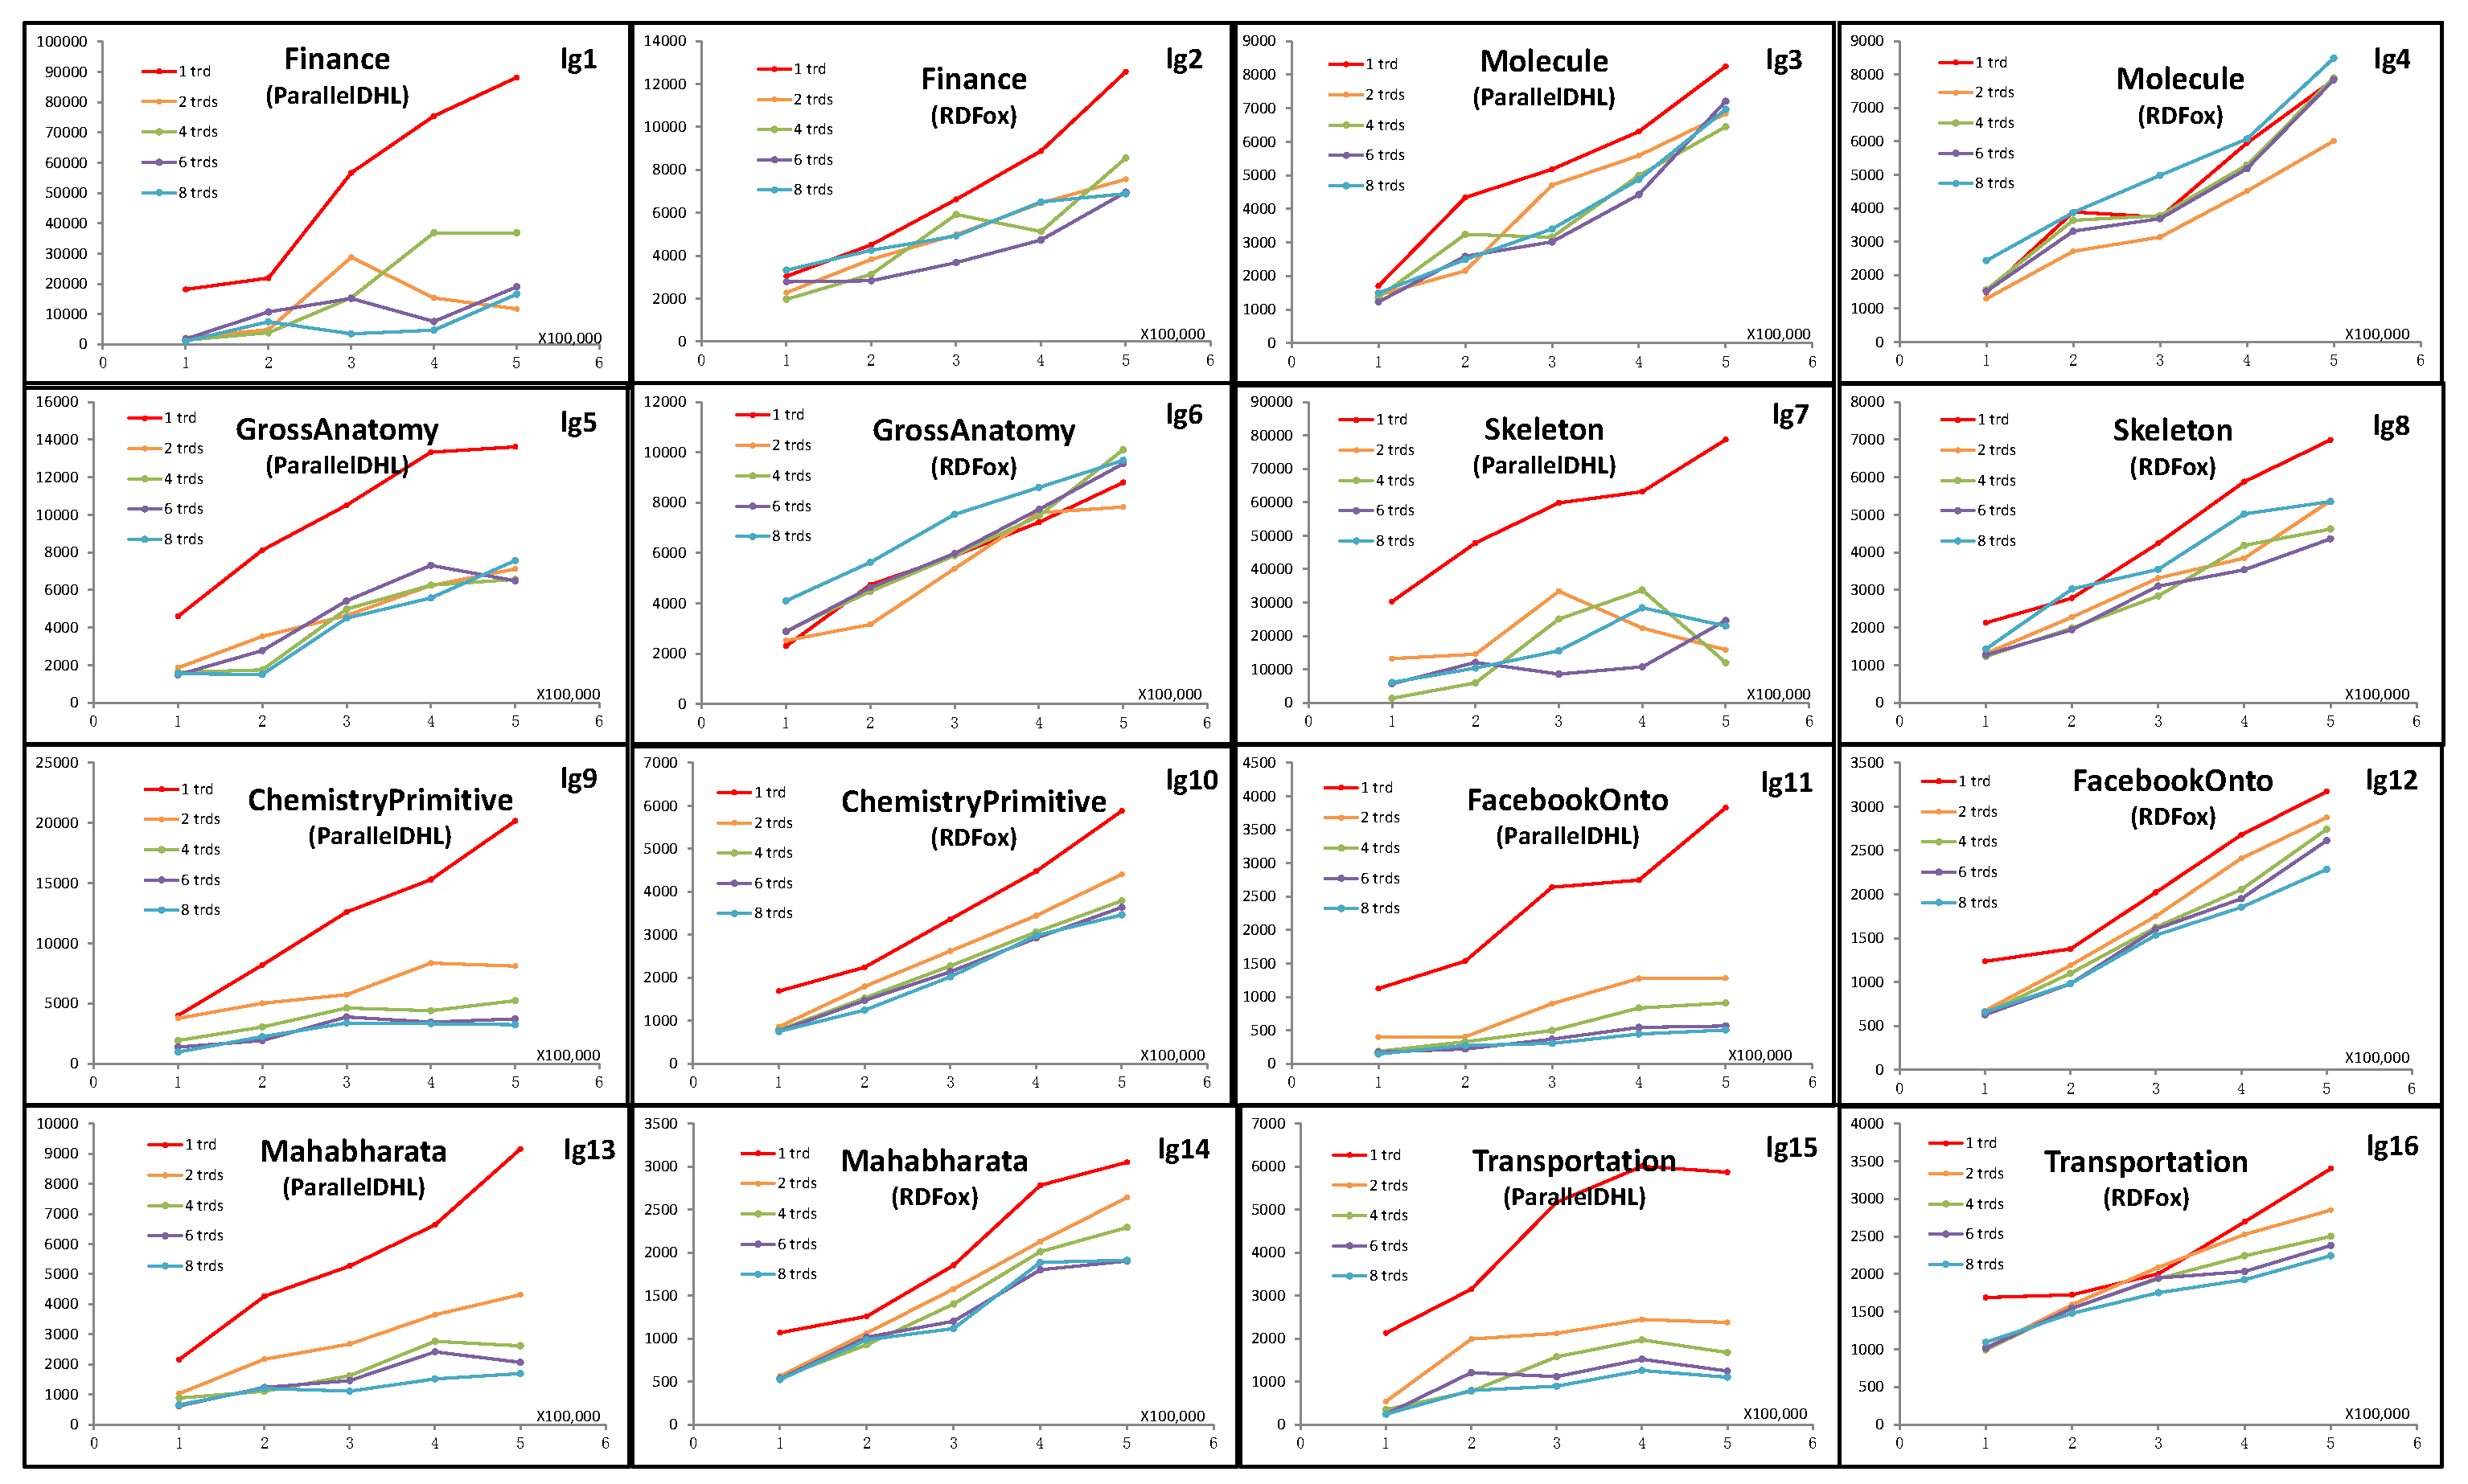
\includegraphics[width=1.5\textwidth,angle=270]{fig-lineGraph.eps}
\caption{The line graphs of all experiments. The 16 line graphs are labeled by $lg1$,...,$lg16$ respectively.}
\label{fig:linegraph}
\end{center}
\end{figure}

\begin{center}
\begin{tabular}{crrrrr}
\multicolumn{6}{c}{\textbf{Table 3: The Analysis of Reasoning Results}}\\
\hline
&~~~~~~~~~~~~~~~1&~~~~~~~~~~~~~~~2&~~~~~~~~~~~~~~~3&~~~~~~~~~~~~~~~4&~~~~~~~~~~~~~~~5\\
\hline
&0.54&1.36&0.94&0.99&1.70\\
Finance&3.06&1.88&2.29&2.95&2.73\\
&1.01&1.04&1.13&1.11&1.19\\
\hline
&0.94&0.79&0.96&0.98&1.07\\
Molecule&1.04&1.24&1.13&1.07&1.05\\
&0.90&1.03&0.95&1.01&0.99\\
\hline
&0.65&0.48&0.84&0.77&0.83\\
GrossAnatomy&1.41&1.69&1.33&1.32&1.22\\
&0.87&0.99&0.94&0.96&0.98\\
\hline
&1.11&\textbf{3.08}&\textbf{3.03}&\textbf{3.04}&\textbf{2.75}\\
Skeleton&3.28&1.84&1.65&1.74&1.96\\
&1.13&1.01&1.06&1.08&1.08\\
\hline
&1.29&1.54&1.68&1.14&0.93\\
ChemistryPrimitive&\textbf{1.46}&\textbf{1.43}&\textbf{1.44}&\textbf{1.51}&\textbf{1.65}\\
&1.28&1.16&1.14&1.11&1.15\\
\hline
&\textbf{0.23}&\textbf{0.22}&\textbf{0.19}&\textbf{0.24}&\textbf{0.22}\\
FacebookOnto&\textbf{1.81}&\textbf{1.83}&\textbf{1.82}&\textbf{1.61}&\textbf{1.78}\\
&1.22&1.08&1.07&1.09&1.09\\
\hline
&1.19&1.19&0.99&0.84&0.89\\
Mahabharata&\textbf{1.41}&\textbf{1.46}&\textbf{1.51}&\textbf{1.47}&\textbf{1.56}\\
&1.24&1.07&1.13&1.10&1.12\\
\hline
&0.24&0.52&0.51&0.65&0.49\\
Transportation&\textbf{1.98}&\textbf{1.57}&\textbf{1.61}&\textbf{1.55}&\textbf{1.59}\\
&1.14&1.04&1.03&1.08&1.11\\
\hline
\end{tabular}
\label{tab:expresult}
\end{center}



%%% Local Variables:
%%% mode: latex
%%% TeX-master: "parallel-tractability-J"
%%% End:
